\chapter{Episodic Logic}

This chapter introduces Episodic Logic (EL), the semantic representation we use in our event schemas. EL's rich temporal semantics make it a natural fit for our schema representation, in which schemas can nest one another to represent compositions of events. Because our schemas are also meant to enable a wide variety of downstream tasks, such as the generation of natural language inferences about the situations represented by unseen stories, EL's structural similarity to the syntax of English is also appealing.

Section~\ref{sec:el} of this chapter introduces EL and discusses its key semantic features. Section~\ref{sec:ulf-parsing} describes ULF, a simplified form of EL meant to act as a stepping stone for EL semantic parsers. That section also describes efforts to parse ULF from English, including our novel, language-model based ULF parser. Finally, in Section~\ref{sec:parsing}, we discuss parsing English sentences into EL given those ULF parses.

%\section{Episodic Logic}

%\section{What's needed for schema learning?}
\label{sec:headstart}
Two components are necessary for schema learning by definition: a model of schemas to learn, and an algorithm to learn them. These cannot be selected independently: as we saw in IPP (Section~\ref{sec:ipp}), the knowledge representation, and the knowledge stored in it, informs even the lowest levels of the learning algorithm, i.e. the syntactic parsing process. A third component that is almost certainly necessary for practical learning is \textit{a priori} common-sense world knowledge: unless one can implement Turing's ``child machine'' \citep{turing1950}---a robot that is a complete ambulatory and sensory facsimile of a human child---schemas must be learned from more indirect sources, like natural language texts, and so some corpus of knowledge is necessary to ``bridge'' purely lexical information with the sorts of observations children would get by virtue of their eyes and ears (e.g. vacuum cleaners are loud, loudness is unpleasant). In other words, we must ``level the playing field'' to give our schema learning systems similar capabilities as the most powerful learning systems we know of: human children.

As my advisor says frequently: \textit{``Babies do not start intellectually as tabulae rasae}\textit{.''} Here, I'll introduce a few capabilities that our group considers to be a necessary ``head start'' for a scalable schema learning system---and some evidence for the presence of these capabilities in actual humans.

\subsection{Symbolic representations}
Although the debate between \textit{connectionist} (i.e. neural, emergent) models of human cognition vs. \textit{classical} (i.e. symbolic, logical) ones rages on, there is evidence that symbolic representations, and symbolic reasoning, exist in the human brain---regardless of the nature of its ``implementation''. In an fMRI study conducted at Purdue \citep{siskind2015}, Jeffrey Mark Siskind's group created a simple space of sentences with 4 possible actors, 3 possible verbs (\textit{carry, fold, leave}), 3 possible objects (\textit{chair, shirt, tortilla}), and 2 directions (\textit{on the left, on the right}), for a total of 72 possible sentences. They recorded videos representing each of these sentences, and took fMRI brain image sequences of human subjects watching these videos.

Using SVM classifiers, they attempted to decode brain image sequences to determine each of the video components independently (actor, verb, object, and direction), as well as the pairs, triples, and full sentences. They were able to determine all combinations of components with accuracy well above chance. Additionally, they trained fMRI classifiers to determine the same set of actions from brain activity when viewing text input \textit{and}, separately, when viewing video input. They were able to get comparable, above-chance accuracy when decoding verbs from images of one modality \textit{using the classifier trained on the other modality}.

Their findings strongly suggest that the brain not only uses compositional action representations (i.e., with ``slots''), but that the areas in the brain that store these representations are common to both text \textit{and} video input---in other words, the brain develops a common symbolic representation of its observations. These results strongly suggest that the brain uses symbols to store information about the world, and these symbols can be generated from many kinds of observation.

\subsection{Slot relationships}
The ``slot-and-filler'' structure of Minsky's frames (see Section~\ref{sec:minsky}) has informed much work on frame-like ontologies. Modern implementations of these frame-like ontologies, such as the description logic \textbf{OWL (Web Ontology Language)} \citep{mcguinness2004owl}, have an analyzable, formal attribute-value semantics, and support slot type constraints, inheritance, composition, and many other useful forms of taxonomic reasoning. However, description logics like \textbf{OWL} do not support the expression of formal, complex \textit{relationships} between their slots: in a frame for a children's school, for example, with slots for a principal and a vice principal, modern frames generally could not formally impose inter-slot constraints such as ``the principal is the boss of the vice principal''. FrameNet (Section~\ref{sec:framenet}) does relate its slots to one another, but only informally, with natural language. Any schema representation we choose to \textit{learn} mechanically should support these sorts of slot relationships with a semantics that can be \textit{reasoned about} mechanically.

\subsection{Branching, conditionals, and variables}
When someone is working to cook a dish, they don't only follow a series of steps. They may have to \textit{branch} (e.g. \textit{if the dough looks wet, lay it on the table and wait five minutes}), execute \textit{loops} (e.g. \textit{check the dough every five minutes, removing it when it appears golden brown}), and manipulate named variables (e.g. \textit{note the weight of the dough in grams; when it's done baking, allow it to cool for half as many minutes as its weight}). In this sense, the schemas that describe our behavior are quite comparable to computer programs, and their representation should facilitate these operations.

\subsection{Time, probability, and meta-reasoning}
Schemas control human behavior in the real world, and so some important aspects of that world should be easily expressible in the language as well. The real world is inherently \textit{temporal}, and so we should be able to express relative times (e.g. \textit{it happened before that}) as well as specified magnitudes (e.g. \textit{it happened two weeks ago}). We also need to express \textit{probabilities and certainties} (e.g. \textit{he has a 50\% chance of winning}, or \textit{it is possible that it will rain tomorrow}). Finally, humans operate in a world with other self-motivated agents, including other humans, and as such must reason about the knowledge and beliefs of others, as well as knowledge transfer mechanisms such as speech. So, whatever form we choose for our schemas should facilitate \textit{attitudinal} inferences such as \textit{John believes that the dough is done}. As we'll see later, certain logical forms have less trouble than others expressing statements of these kinds.
    
\subsection{Analog representations}
Although Minsky discusses applying symbolic frames to 3D scene understanding, human beings seem to have especially strong, unconscious intuitions about certain physical and spatial properties. 3D object representations are suspected to be analog in humans, that is, in some sort of spatial correspondence with the objects themselves: the time humans take to mentally rotate 3D images is proportional to the degree of rotation \citep{cooper1973chronometric}. Additionally, object representation is suspected to occur largely in a dedicated brain area \citep{rosenberg2013visual}. Spatial reasoning is an extremely important aspect of story understanding, as stories take place in a physical world. And, owing to the computational difficulty of spatial reasoning, we should try to separate these ``specialist'' systems from the symbolic machinery, and optimize them independently, to whatever extent we can.
    
\subsection{Behavioral axioms}
\label{sec:schema_behavior}
Even human newborns cry for food. This is notable: being hungry is unpleasant, and even in the earliest days of their lives, human beings are ``pre-programmed'' with desires to avoid certain displeasures, to seek certain rewards, and to pursue actions---even highly primitive, instinctive ones like crying---that help realize those desires. This kind of ingrained tendency toward goal-driven action is central to understanding one's own actions, as well as the actions of others.
    
\subsection{Primitive actions}
\label{sec:schema_primitives}
OK, \citep{schank1975concdep} may have something of a point. There do seem to be certain primitive actions---crying, laughing, grasping, holding, eating---that infants start out with, experiment with, and compose to achieve basic goals. However, the key distinction from the primitive actions of Schank's CD theory is that these actions form a \textit{``starter pack''}, rather than an \textit{atomic representation}: one cannot compose all actions from what babies know how to do, and, even in the cases where one can, one still does not conceptualize complex actions like ``fishing'' in terms of thousands of separate grasping actions. However, some basic actions do seem to give a good head start to infants.
    
\subsection{Language learning}
Young humans acquire language rapidly, and language can then be used to learn nearly arbitrary information. Siskind's work, described above, suggests that our linguistic representations are split into symbols that are then used to represent entities and actions across verbal and visual modalities. Language is important for learning---especially when your goal is to learn from texts, which are more plentiful, and arguably easier to extract features from, than richer modalities such as videos.

\section{Implementing what's needed}
Imbuing a computer with any of the capabilities listed above is no small task, but learning them from scratch in a neural model seems especially daunting: how could we acquire the data needed to learn these things at the scale needed to cover the vast number of possible situations that exist? Our research group, led by Lenhart Schubert at the University of Rochester, is pursuing alternative approaches to constructing this ``head start'', such that schema learning can proceed from a small number of examples (relative to the data needed to train neural networks). Georgiy Platonov is pursuing computational understanding of spatial descriptions \citep{platonov2018computational}; Gene Kim is developing a semantic parser for mapping English to an intermediate semantic representation that directly enables certain discourse inferences while also providing a starting point for transduction into a nonindexical\footnote{Details of what this means are available in \citep{kim2019type}; here, I'll just say that ``deindexing'' includes tasks like converting the speaker-relative tense information in sentences to explicit, atemporal statements about individual episodes.} logical language \citep{kim2019type}; and together with his students, Lenhart Schubert has spent years developing that formal logical language, known as \textbf{Episodic Logic (EL)} \citep{hwang1993}, hypothesizing that the semantic types available in this language are the ones innate in human ``mentalese''.

As I join my advisor and colleagues to pursue the eventual goal of scalable schema acquisition, I will---and, in fact, have already begun to---make heavy use of Episodic Logic to define a schema representation and enable powerful inferences on, and generalizations of, schemas in that representation. So, before I detail our approach to the schema learning problem, and the work I've done toward that approach so far, I will briefly describe EL.

\section{Episodic Logic (EL)}
\label{sec:el}

EL is a predicate logic whose semantics are intended to model some important aspects of natural language, and of the human thought patterns that give rise to natural language.  As its name implies, one of EL's most distinctive features is its \textit{characterization} operator, \texttt{**}, which relates possible situations (a.k.a. \textit{episodes}, which include what we would informally call events) to the logical propositions that characterize them. EL also maps predicate and propositional intensions to \textit{individuals} within its logical domain; these intensional individuals are formed from EL's predicates and propositions using reification operators. Proposition intensions, when reified to individuals, can act as arguments to intensional verb predicates, e.g., \textit{believe} and \textit{resemble}. Predicate intensions can also be type-shifted into complex predicate \textit{modifiers}, e.g., \textit{hopefully believable}. EL also avoids a Montague-style treatment of determiners as second-order predicates, instead providing generalized, restricted quantifiers, including nonstandard quantifiers, e.g., \textit{most of the older boys}.

\begin{figure}
    \centering
    \resizebox{\columnwidth}{!}{
    \vbox{
    % Made with matchcha.io---strong recommendation from me! :)

%\epigraph{\textit{There are more things in heaven and earth, Horatio, Than are dreamt of in your philosophy.}}{---William Shakespeare, \textit{Hamlet}}

\tikzset{every picture/.style={line width=0.75pt}} %set default line width to 0.75pt        

\begin{center}
\scalebox{1.0}{
\makebox[\textwidth][c]{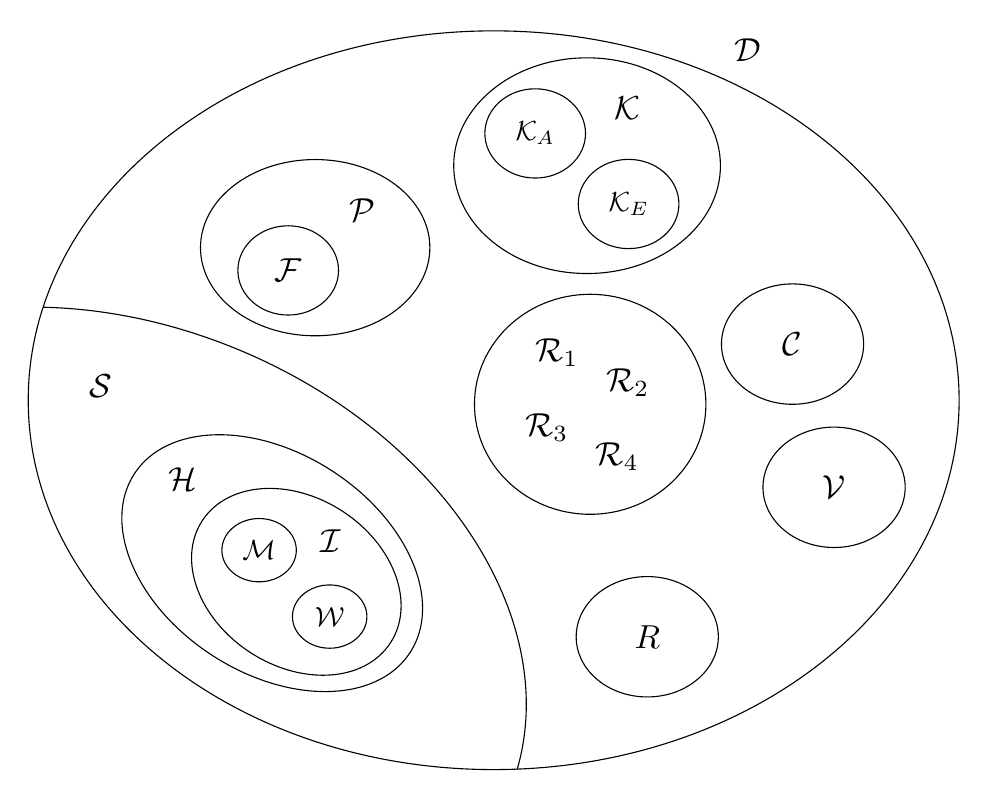
\begin{tikzpicture}[x=0.75pt,y=0.75pt,yscale=-1,xscale=1,scale=1,every node/.style={scale=1}]
%uncomment if require: \path (0,721.921875); %set diagram left start at 0, and has height of 721.921875

%Shape: Ellipse [id:dp9100065238827619] 
\draw   (98,300.96) .. controls (98,202.68) and (198.4,123) .. (322.25,123) .. controls (446.1,123) and (546.5,202.68) .. (546.5,300.96) .. controls (546.5,399.25) and (446.1,478.92) .. (322.25,478.92) .. controls (198.4,478.92) and (98,399.25) .. (98,300.96) -- cycle ;
%Shape: Ellipse [id:dp10388374342633644] 
\draw   (181,227.46) .. controls (181,204.01) and (205.74,185) .. (236.25,185) .. controls (266.76,185) and (291.5,204.01) .. (291.5,227.46) .. controls (291.5,250.91) and (266.76,269.92) .. (236.25,269.92) .. controls (205.74,269.92) and (181,250.91) .. (181,227.46) -- cycle ;
%Shape: Ellipse [id:dp27736097111625835] 
\draw   (199,238.42) .. controls (199,226.55) and (209.86,216.92) .. (223.25,216.92) .. controls (236.64,216.92) and (247.5,226.55) .. (247.5,238.42) .. controls (247.5,250.3) and (236.64,259.92) .. (223.25,259.92) .. controls (209.86,259.92) and (199,250.3) .. (199,238.42) -- cycle ;
%Shape: Ellipse [id:dp7888799168086817] 
\draw   (303,187.96) .. controls (303,159.26) and (331.77,136) .. (367.25,136) .. controls (402.73,136) and (431.5,159.26) .. (431.5,187.96) .. controls (431.5,216.66) and (402.73,239.92) .. (367.25,239.92) .. controls (331.77,239.92) and (303,216.66) .. (303,187.96) -- cycle ;
%Shape: Ellipse [id:dp4804121479534271] 
\draw   (363,206.42) .. controls (363,194.55) and (373.86,184.92) .. (387.25,184.92) .. controls (400.64,184.92) and (411.5,194.55) .. (411.5,206.42) .. controls (411.5,218.3) and (400.64,227.92) .. (387.25,227.92) .. controls (373.86,227.92) and (363,218.3) .. (363,206.42) -- cycle ;
%Shape: Ellipse [id:dp0795716353230258] 
\draw   (318,172.42) .. controls (318,160.55) and (328.86,150.92) .. (342.25,150.92) .. controls (355.64,150.92) and (366.5,160.55) .. (366.5,172.42) .. controls (366.5,184.3) and (355.64,193.92) .. (342.25,193.92) .. controls (328.86,193.92) and (318,184.3) .. (318,172.42) -- cycle ;
%Shape: Ellipse [id:dp12618348576003102] 
\draw   (432,273.92) .. controls (432,257.91) and (447.33,244.92) .. (466.25,244.92) .. controls (485.17,244.92) and (500.5,257.91) .. (500.5,273.92) .. controls (500.5,289.94) and (485.17,302.92) .. (466.25,302.92) .. controls (447.33,302.92) and (432,289.94) .. (432,273.92) -- cycle ;
%Shape: Ellipse [id:dp8799691211755756] 
\draw   (452,342.92) .. controls (452,326.91) and (467.33,313.92) .. (486.25,313.92) .. controls (505.17,313.92) and (520.5,326.91) .. (520.5,342.92) .. controls (520.5,358.94) and (505.17,371.92) .. (486.25,371.92) .. controls (467.33,371.92) and (452,358.94) .. (452,342.92) -- cycle ;
%Shape: Ellipse [id:dp824996442524188] 
\draw   (362,414.92) .. controls (362,398.91) and (377.33,385.92) .. (396.25,385.92) .. controls (415.17,385.92) and (430.5,398.91) .. (430.5,414.92) .. controls (430.5,430.94) and (415.17,443.92) .. (396.25,443.92) .. controls (377.33,443.92) and (362,430.94) .. (362,414.92) -- cycle ;
%Shape: Ellipse [id:dp8272383634329143] 
\draw   (313,302.92) .. controls (313,273.65) and (337.96,249.92) .. (368.75,249.92) .. controls (399.54,249.92) and (424.5,273.65) .. (424.5,302.92) .. controls (424.5,332.19) and (399.54,355.92) .. (368.75,355.92) .. controls (337.96,355.92) and (313,332.19) .. (313,302.92) -- cycle ;
%Shape: Arc [id:dp39537977602891705] 
\draw  [draw opacity=0] (105.32,256.16) .. controls (135.93,256.87) and (168.45,263.64) .. (200.4,277.07) .. controls (297.72,317.98) and (354.69,406) .. (333.59,478.73) -- (143.5,412.42) -- cycle ; \draw   (105.32,256.16) .. controls (135.93,256.87) and (168.45,263.64) .. (200.4,277.07) .. controls (297.72,317.98) and (354.69,406) .. (333.59,478.73) ;
%Shape: Ellipse [id:dp5287011551360823] 
\draw   (149.07,336.49) .. controls (164.96,311.91) and (207.6,311.22) .. (244.32,334.95) .. controls (281.04,358.69) and (297.92,397.86) .. (282.03,422.44) .. controls (266.14,447.02) and (223.49,447.71) .. (186.77,423.97) .. controls (150.06,400.24) and (133.18,361.07) .. (149.07,336.49) -- cycle ;
%Shape: Ellipse [id:dp015166695228427951] 
\draw   (181.78,359.11) .. controls (193.96,340.26) and (224.16,338.12) .. (249.23,354.32) .. controls (274.3,370.53) and (284.75,398.94) .. (272.56,417.79) .. controls (260.38,436.64) and (230.18,438.78) .. (205.11,422.58) .. controls (180.04,406.37) and (169.59,377.96) .. (181.78,359.11) -- cycle ;
%Shape: Ellipse [id:dp4822793325306267] 
\draw   (191.3,373.21) .. controls (191.3,364.79) and (199.33,357.96) .. (209.23,357.96) .. controls (219.14,357.96) and (227.17,364.79) .. (227.17,373.21) .. controls (227.17,381.63) and (219.14,388.45) .. (209.23,388.45) .. controls (199.33,388.45) and (191.3,381.63) .. (191.3,373.21) -- cycle ;
%Shape: Ellipse [id:dp37988107849014874] 
\draw   (225.3,405.21) .. controls (225.3,396.79) and (233.33,389.96) .. (243.23,389.96) .. controls (253.14,389.96) and (261.17,396.79) .. (261.17,405.21) .. controls (261.17,413.63) and (253.14,420.45) .. (243.23,420.45) .. controls (233.33,420.45) and (225.3,413.63) .. (225.3,405.21) -- cycle ;

% Text Node
\draw (133,294) node [scale=1.2]  {$\mathcal{S}$};
% Text Node
\draw (244,369) node [scale=1.2]  {$\mathcal{I}$};
% Text Node
\draw (209.23,373.21) node [scale=1]  {$\mathcal{M}$};
% Text Node
\draw (243.23,405.21) node [scale=1]  {$\mathcal{W}$};
% Text Node
\draw (172.23,339.21) node [scale=1.2]  {$\mathcal{H}$};
% Text Node
\draw (396.25,414.92) node [scale=1.2]  {$\mathbb{R}$};
% Text Node
\draw (352.8,278.27) node [scale=1.2]  {$\mathcal{R}_{1}$};
% Text Node
\draw (386.8,292.27) node [scale=1.2]  {$\mathcal{R}_{2}$};
% Text Node
\draw (347.8,314.27) node [scale=1.2]  {$\mathcal{R}_{3}$};
% Text Node
\draw (381.8,328.27) node [scale=1.2]  {$\mathcal{R}_{4}$};
% Text Node
\draw (386.8,160.27) node [scale=1.2]  {$\mathcal{K}$};
% Text Node
\draw (342.25,172.42) node [scale=1]  {$\mathcal{K}_{A}$};
% Text Node
\draw (387.25,206.42) node [scale=1]  {$\mathcal{K}_{E}$};
% Text Node
\draw (466.25,273.92) node [scale=1.2]  {$\mathcal{C}$};
% Text Node
\draw (486.25,342.92) node [scale=1.2]  {$\mathcal{V}$};
% Text Node
\draw (258.8,209.27) node [scale=1.2]  {$\mathcal{P}$};
% Text Node
\draw (223.25,238.42) node [scale=1.2]  {$\mathcal{F}$};
% Text Node
\draw (444.8,132.27) node [scale=1.2]  {$\mathcal{D}$};


\end{tikzpicture}}}
\end{center}

\small
\makebox[\textwidth][c]{\begin{tabular}{c c l}
   & & \\
   $\mathcal{D}$  & & The full \textit{domain} of EL individuals; the union of all following sets \\
   $\mathcal{S}$  & & Possible situations, a.k.a. \textit{episodes}, forming a join semilattice in any given possible world \\
   $\mathcal{H}$  & & Informationally-maximal episodes, a.k.a. \textit{exhaustive situations} \\
   $\mathcal{I}$  & & Spatially-maximal exhaustive situations, a.k.a. \textit{possible times}, a.k.a intervals \\
   $\mathcal{W}$  & & Spatiotemporally-maximal intervals, a.k.a. \textit{possible worlds} \\
   $\mathcal{M}$  & & Spatially-maximal, temporally-minimal intervals, a.k.a. \textit{moments of time} \\
   $\mathcal{P}$  & & \textit{Propositions} \\
   $\mathcal{F}$  & & Consistent propositions, a.k.a. \textit{possible facts} \\
   $\mathcal{K}$  & & \textit{Kinds of individuals}, whose realizations are ordinary individuals \\
   $\mathcal{K}_{A}$  & & \textit{Kinds of actions}, whose realizations are pairs of ordinary individuals and situations \\
   $\mathcal{K}_{E}$  & & \textit{Kinds of episodes}, whose realizations are situations for which a particular characterization holds \\
   $\mathcal{C}$  & & \textit{Collections} of individuals \\
   $\mathcal{V}$  & & \textit{$n$-tuples} of individuals, $n \geq 2$ \\
   $\mathbb{R}$  & & \textit{The real numbers} \\
   $\mathcal{R}_{1}$  & & \textit{Clock times, a uniformly discretized subset of $\mathbb{R}$}, containing subsets of $\mathbb{R}_{n}$
   %& & Note that $\mathcal{R}_{4}$, which represents space-time regions, contains some unconnected \\
   %& & space-time trajectories; these trajectories describe the time and place of episodes.
\end{tabular}}
    }
    }

    \caption{A representation of the EL ontology. I include only some brief definitions of its notable subsets; for more formal detail, please refer to \citep{schubert2000episodic}.}% \tiny{(I'd like to thank \href{https://www.mathcha.io}{mathcha.io} for making the construction of this TikZ figure so painless with their graphical editor.)}}
    \label{fig:el_ontology}
\end{figure}

The EL ontology of individuals, represented by Figure~\ref{fig:el_ontology}, gives a hierarchical organization of the basic semantic types of EL. The \textit{kind-forming} operators---$\texttt{K}$ (kind), $\texttt{KA}$ (kind of action), and $\texttt{KE}$ (kind of event)---reify predicates and propositions into the respectively named types in the ontology. EL defines a variety of semantic types, such as those for predicates and modifiers, on the basis the domain of individuals $\mathcal{D}$, and the set of truth values, $\{0,1\}$, also written as \textbf{2}. These semantic types are compositions of mapping functions, each of which is notated $(X \rightarrow Y)$ to mean a function mapping set $X$ to set $Y$. For example, the monadic noun predicate \texttt{STEAK.N}, denoting the set of individuals that are steak, has semantic type $(\mathcal{D} \rightarrow (\mathcal{S} \rightarrow \textbf{2}))$: it is a mapping of individuals to mappings of \textit{situations} to truth values, thereby affording intensionality. $n$-adic predicates generally have the type $(\mathcal{D}^{n} \rightarrow (\mathcal{S} \rightarrow \textbf{2}))$. Semantic types in EL may be re-cast using \textit{type-shifting} operators, e.g., the reifying operator \texttt{K}, a.k.a. the \textit{kind} operator, which maps a monadic predicate into a ``kind of'' individual and has semantic type $((\mathcal{D} \rightarrow (\mathcal{S} \rightarrow \textbf{2})) \rightarrow \mathcal{K})$.

\subsection{Examination of an Example}
In lieu of formal, detailed definitions of all of EL's features, which can be found in \citep{schubert2000episodic} \footnote{modulo a redefinition of the semantics of the characterizing operator, \el{**}, in terms of the underlying predicate semantics \citep{len-situations-2000} instead of the semantics of the truth-in operator, \el{*}}, the remainder of this section is dedicated to the examination of an example of an English/EL pair that illustrates some of those most notable features. Everything heretofore written in this section will refer to the formula in Figure~\ref{fig:eng_el_pair}.

\subsubsection{The \el{**} operator}
Two propositions \textit{characterize} event individuals in the example formula: the \el{insist.v} proposition, which characterizes \el{e1.sk}, and the \el{like.v} proposition, which characterizes \el{e2}. When a formula $\phi$ characterizes an episode \el{e}, it means that \el{e} is \textit{an episode of} $\phi$, e.g., an episode of Mary liking art; we write this relationship as \el{($\phi$ ** e)}. The characterization of episode individuals by formulas is similar to the Davidsonian notion of events \citep{Davidson1967}, where an event is a first-class domain entity passed as an extra argument to situational predicates. Davidsonian event variables, however, may only passed to positive, atomic predications; Episodic Logic's semantics allow arbitrarily complex formulas to characterize, and thus to hold in certain events.

\el{**} is a \textit{modal} operator: statements like \el{[$\phi$ ** e]} may not, in general, have their formula argument, $\phi$, replaced with other formulas that seem to have the same truth value. So, the EL formula \el{((|Andre| sleep.v) ** e)} does \textit{not} entail \el{(((|Andre| sleep.v) $\land$ ( (|Fido| bark.v) $\lor$ $\neg$ (|Fido| bark.v) )) ** e)}, even though it has the same truth value; in fact, the entity \el{|Fido|} might not have any role in the episode, and so even tautological statements involving it may have no truth value in \el{e}.

\begin{figure}

\textbf{English}: \textit{Most of the senior students will insist that they liked art.}

\textbf{EL}: \begin{lstlisting}[xleftmargin=4.5em,style=EL,mathescape=true]
(e1.sk after Now) $\land$
(most.det x [(x student.n) $\land$ (x senior.a)]
    ((x insist.v (that 
        ($\exists$ e2 [e2 before e1.sk]
            ( (x like.v (k art.n)) ** e2 )
                ))) ** e1.sk))
\end{lstlisting}
    \caption{An example of an English sentence and its EL interpretation. There is no difference, here, between square brackets and parentheses; they alternate only to make distinguishing certain clauses easier. Note that, in this notation, each subject argument \textit{precedes} its predicates, while all other arguments follow the predicate. In the ``curried'' semantics, subject arguments come last.}
    \label{fig:eng_el_pair}
\end{figure}

\subsubsection{Restricted quantification}
The existential quantification of \el{e2}\footnote{e1.sk, on the other hand, is a Skolem constant---it has been assigned a name to remove the top-level existential quantification of \el{e1}. \el{e2} could not be similarly Skolemized, as it is within the scope of the intensional predicate \texttt{insist.v}. Even without this intensional scope, though, \el{e2} would still have a subscope dependency on the quantified value of \el{x}, i.e., \el{e2} would be a Skolem function of \el{x}.} illustrates the ``restrictor-matrix'' structure of EL quantification: if \el{x} is a variable, \el{Q} is a quantifier, and $\phi$ and $\psi$ are arbitrary EL formulas, the quantification formula \el{[Q x : $\phi$ $\psi$]} predicates the truth of the ``matrix'' formula $\psi$ in quantification cases where the ``restrictor'' formula $\phi$ holds true. When \el{Q} is $\exists$, this is equivalent to the unrestricted quantification \el{[$\exists$ x ($\phi \land \psi$)]}; similarly, when \el{Q} is $\forall$, it is equivalent to \el{[$\forall$ x ($\phi \rightarrow \psi$)]}. However, as can be seen in the quantification of \el{x} by the quantifier \el{most.det}, not all quantifiers can be simplified in this way: nonstandard quantifiers like \textit{most}, \textit{many}, and \textit{few} do not permit conjunctive or implicative re-writing of the restrictor formula.

\subsubsection{Temporal relations}
The temporal relation \el{before} is used to relate the time of \el{e1.sk} to the special time constant \el{now}---which represents the time that the speaker is uttering the sentence---and the time of \el{e2} to \el{e1.sk}, and thus also \el{e2} to \el{now}.
As \el{now} is indexical by default, if more than one utterance exists, we ``timestamp'' each utterance's \el{now}, e.g., \el{Now1}.
Such temporal relations---as well as the tacit temporal relations in their transitive closures---allow projection of the episodes onto temporal intervals within the ontological domain $\mathcal{R}_{1}$, representing discretized times (see Figure~\ref{fig:el_ontology}).
%Not all spacetime trajectories are transitively connected, however; the intensional environment of the verb predicate \el{insist.v} implies a new set of possible situations for the truth of the \el{like.v} proposition characterizing \el{e2}.

More temporal relations exist, special functions \el{start-of(e)} and \el{end-of(e)} allow temporal predications about the instantaneous endpoints of episodes, and disjoint intervals may even form an episode (e.g., \textit{Andre sneezed repeatedly}); for more information on the temporal semantics of EL, please refer to the original semantics due to \citet{hwang1993episodic} and their revisions by \citet{len-situations-2000}.

\subsubsection{Reification and \textit{kind}-forming}
The kind-forming operator \el{K} is used here because \el{art.n} is a one-place predicate that determines whether its argument is ``art''. Because the speaker does not have any specific art in mind, we choose to make a statement about the students liking the \textit{kind of thing} ``art'', which we accomplish by \textit{reifying} the \el{art.n} predicate, rather than \textit{Skolemizing} a variable (i.e., assigning it a concrete name, to bypass existential quantification) and attaching the predicate to it (i.e., assigning it a name). In order to use a predicate as an argument to another predicate, we must first reify it as an individual.

Reification can also be performed on other types of predicates. The reified verb phrase \el{(Ka (drink.v (K water.n)))}
%\footnote{What's being reified is actually not a well-formed EL predication, assuming \el{drink.v} is a 2-place predicate; the actor argument is missing! What's \textit{actually} being reified here, implicitly using the \el{K} operator, is something like the \textit{lambda abstraction} \el{($\lambda$a (a drink.v (K water.n)))}; however, even that's not quite right, as there are additional complications related to event characterization. For a full discussion of this, see page 7 of \citep{schubert2000episodic}.}
is the \textit{kind of action} of drinking water, and belongs to the class $\mathcal{K}_{A}$ in the EL ontology (see Figure~\ref{fig:el_ontology}), whose realizations are (individual, episode) pairs.
What's being reified by the \el{Ka} operator is a well-formed monadic EL predication, assuming \el{drink.v} is a 2-place ``curried'' predicate; \el{Ka} can be defined in terms of the \el{K} operator as \el{(K ($\lambda$a (((1st a) drink.v (K water.n)) ** (2nd a))))}, which is a kind whose realizations \el{a} have an agent as the first element and an episode as the second element. \footnote{see page 7 of \citep{schubert2000episodic}}
The reified sentence \el{(Ke (|Mary| drink.v (K water.n)))} is the \textit{kind of event} where Mary drinks water, and belongs to the ontological class $\mathcal{K}_{E}$. The \el{Ke} operator can also be defined in terms of the \el{K} operator: \el{(Ke $\phi$)} = \el{(K $\lambda$e ($\phi$ ** e))}. \el{Ke}-reification is semantically distinct from the other reification of this sentence, which uses the \el{That} operator, \el{(That (|Mary| drink.v (K water.n)))}, which is a \textit{proposition}, and thus belongs to the ontological class $\mathcal{P}$. An intuition for their semantic distinction is quite easy to obtain from the names of their operators: ``the kind of event of Mary drinking water'' is obviously different from the proposition ``that Mary is drinking water''.
%However, the restrictor-matrix form cannot be simplified in this manner for some of EL's nonstandard quantifiers, e.g., \el{Most}.
%As its name implies, one of EL's most distinctive features is its use of \textit{episode} variables to denote time-bounded ``temporal'' propositions, such as ``Palutena is sleepy'' or ``I'll go running for an hour''---as well as ``atemporal'' propositions, which necessarily hold true eternally, like ``hydrogen is an element'' or $2+3=5$.

%EL naturally supports other aspects of natural language as well. It is an \textit{intensional} logic: a sentence like ``Gaurav loves Mariel'' can represented as not just a truth value, but as a function from possible situations to truth values called a \textit{sentence intension}. Sentence intensions may be transmuted into individuals using \textit{reification} operator \texttt{That}, and predicates may be similarly reified into individuals with the kind-forming operator \texttt{K}\footnote{Or \texttt{Ke} for forming kinds of events, or \texttt{Ka} for forming kinds of actions.}; this allows abstract entities, such as \textit{``the process of writing a dissertation''}, as well as concrete entities, such as \textit{``Lane's dissertation''}, to act as predicate arguments without defining special semantics for higher-order predicates (that is, predicates with predicate arguments).

\section{ULF Parsing}

\begin{figure}
\centering
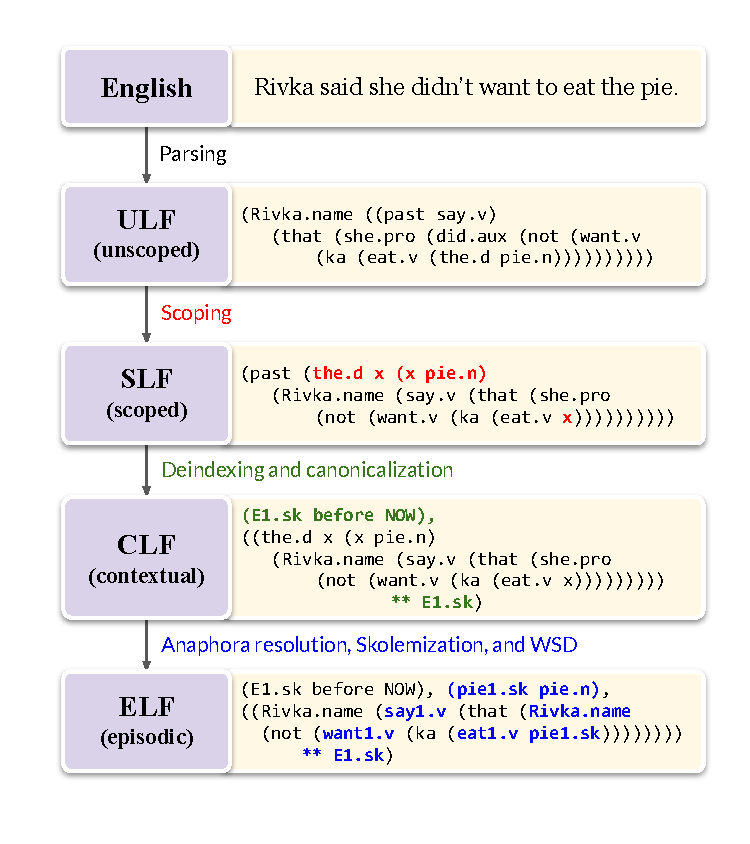
\includegraphics[width=\columnwidth]{CH2_el/el_pipeline.pdf}
\label{fig:el_pipeline}
\caption{The stages of the Episodic Logic parsing pipeline. Solid arrows represent the flow of data through the pipeline, and are labeled with the steps needed to obtain the target forms. The relevant changes are highlighted in each stage's example.}
\end{figure}

\label{subsec:ulf}
Unscoped Logical Form (ULF), an intermediate form of Episodic Logic, formally represents the semantic types and predicate-argument structures of natural language. It is the first, and most developed, step in the ``divide and conquer'' approach to EL parsing illustrated in Figure~\ref{fig:el_pipeline}. In order to obtain ELFs from ULFs, one must, at the very least, perform quantifier scoping, resolve anaphora, deindex the temporal coordinates of events, and disambiguate word senses, and \textit{canonicalization} (the minimization of ELFs into separate propositions by Skolemizing existentially quantified variables at the top level).

\citet{kim2022corpus} fully describes ULF and the current state of ULF parsing. In this section, we describe our language model-based ULF parser \citep{gibson2022language} and evaluate it against two other ULF parsers: a symbolic, rule-based transduction from constituency parses \citep{kim2021naloma} and a neural cache transition parser \citep{kim2021transition}, ultimately justifying our choice of the rule-based transduction method.

\subsection{Language Model-Based ULF Parsing}
In crafting an EL parsing pipeline, we experimented with using GPT-2, a state-of-the-art language model architecture based on a decoder-only transformer \citep{Radford2019LanguageMA}. Our intuition was that, given ULF's similarity to the syntactic surface form of English, a pre-trained language model might be able to perform well at ULF parsing by casting the problem as one of translation. In this light, we fine-tuned GPT-2 models to perform translation not just of English into ULF (parsing), but of ULF into English (verbalization). This section describes those models and the experiments performed on them.
\subsubsection{Objective}
%Like \citet{gpt-too}, we chose to fine-tune the GPT-2 \citep{Radford2019LanguageMA} language model to perform both of our tasks. Our approach differs slightly in that we did not adapt the default tokenizer to the ULF syntax, nor did we add the \texttt{\textbf{<SEP>}} or \texttt{\textbf{<END>}} tokens to the GPT-2 vocabulary, as modifying the tokenizer did not meaningfully improve performance on either task.
Given a tokenized English sentence $e = e_{1} \cdot e_{2} \cdot \ldots \cdot e_{m}$ and a tokenized s-expression representation of a corresponding ULF $u = u_{1} \cdot u_{2} \cdot \ldots \cdot u_{n}$, we fine-tuned our English-to-ULF GPT2 model for 327 epochs to maximize the joint probability of the concatenated sequences \footnote{The special tokens \texttt{<SEP>} and \texttt{<END>} were included between and after the two concatenated sequences, respectively, for every pair in the dataset.} $e$ and $u$, $P_{\textrm{GPT2}}(u,e) = P_{\textrm{GPT2}}(u|e) \cdot P_{\textrm{GPT2}}(e)$, where:

\vspace{3mm}

$$\mathlarger{P_{\textrm{GPT2}}(u|e) = \prod_{i=1}^{n} P_{\textrm{GPT2}}(u_{i} | e_{1:m},u_{1:i-1})}$$
\vspace{1mm}

$$\mathlarger{P_{\textrm{GPT2}}(e) = \prod_{j=1}^{m} P_{\textrm{GPT2}}(e_{j} | e_{1:j-1})}$$

\vspace{3mm}

The maximization objective for the ULF-to-English verbalization model is obtained by instead decomposing the joint probability $P_{\textrm{GPT2}}(u,e)$ into the similarly defined $P_{\textrm{GPT2}}(e|u)$ and $P_{\textrm{GPT2}}(u)$.

\subsubsection{Dataset}

We used the hand-annotated ULF dataset provided by \citet{kim2021transition}, comprising 1,738 sentences. We split our training (1,378), development (180), and test (180) sentences as prescribed in that paper. The data splitting aims to evenly distribute document-level topics among each subset of the sentences, and to avoid score inflation from linguistic similarity between adjacent sentences.

%For each English-ULF pair in the dataset, we produced fine-tuning data as seen in Figure~\ref{fig:dataset}.
To fine-tune the language model on these pairs, we constructed for each pair a tokenized English sentence $e = e_{1} \cdot e_{2} \cdot \ldots \cdot e_{m}$ and a tokenized s-expression representation of the corresponding ULF $u = u_{1} \cdot u_{2} \cdot \ldots \cdot u_{n}$. We fine-tuned our English-to-ULF and ULF-to-English GPT-2 models to maximize the joint probability of the concatenated sequences. \footnote{The special tokens \texttt{<SEP>} and \texttt{<END>} were included between and after the two concatenated sequences, respectively, for every pair in the dataset.}

To obtain each task's final model, we used the Huggingface transformer library to fine-tune the 774M-parameter \texttt{gpt2-large} model for 327 epochs with a block size of 128.

\subsubsection{Generation}

The trained model yields probability distributions over all tokens for each element in the output sequence ($\hat{e}_{i}$ for generated English and $\hat{u}_{j}$ for generated ULF). We experimented with several decoding methods for obtaining output strings from these probability distributions. As \citet{gpt-too} did, we evaluated generations for both tasks decoded using beam search, greedy sampling, nucleus (top-$p$) sampling.

We additionally evaluated generations decoded using thermal sampling, where, prior to a weighted random token selection, $p_{i,t}$, the probability of each token $t$ at each position $i$, is transformed according to $\tilde{p}_{i,t} = p_{i,t}^{\frac{1}{\tau}}\ /\ \sum_{j} p_{i, t}^{\frac{1}{\tau}}$, controlled by the temperature parameter $\tau$. When $\tau = 0$, thermal sampling is equivalent to greedy sampling.

For the verbalization model, all decoding methods were evaluated with and without the \elsmatch re-scoring described in Section~\ref{subsec:rescoring}; the results are presented in Table~\ref{T3}, and support the choice of the 10-beam, non-rescored decoder for the comparisons to other parsers in Section~\ref{subsec:ulf-eval}. For the parsing model, we used the same choice of decoder.

\vspace{5mm}

\begin{table}[ht]
\centering
\begin{tabular}{l|c|c|c}
\toprule
\multicolumn{1}{c|}{\textbf{Model}}&\multicolumn{1}{c|}{\textbf{BLEU}}&\multicolumn{1}{c|}{\textbf{chrF++}}&\multicolumn{1}{c}{\textbf{METEOR}}\\
% \textbf{CORA}&\textbf{Citeseer}&\textbf{Pubmed}
%\midrule
%Model&Accuracy&Accuracy&Accuracy\\
\midrule
\texttt{Greedy}&0.67&0.81&0.76\\
\texttt{Greedy (els)}&0.67&0.81&0.76\\
\texttt{Beam 10}&\textbf{0.72}&\textbf{0.84}&\textbf{0.80}\\
\texttt{Beam 10 (els)}&\textbf{0.72}&\textbf{0.84}&\textbf{0.80}\\
\texttt{Beam 15}&\textbf{0.72}&\textbf{0.84}&\textbf{0.80}\\
\texttt{Beam 15 (els)}&\textbf{0.72}&\textbf{0.84}&\textbf{0.80}\\
\texttt{Nucleus}&0.68&0.82&0.77\\
\texttt{Nucleus (els)}&0.68&0.82&0.78\\
\texttt{Temp 0.5}&0.69&0.82&0.77\\
\texttt{Temp 0.5 (els)}&0.71&\textbf{0.84}&0.79\\
\texttt{Temp 1.0}&0.67&0.81&0.77\\
\texttt{Temp 1.0 (els)}&0.66&0.81&0.77\\
\bottomrule
\end{tabular}\\[10pt]
\caption{Results for all decoding methods in our ULF-to-English verbalization model, with and without an \elsmatch re-scoring term (\texttt{els}) added to the generated log probability. All scores are out of 1.0.\label{T3}}
\end{table}

\subsubsection{Sample Re-Scoring for Verbalizations}
\label{subsec:rescoring}
In \citep{gpt-too}, the top K generated ULF formulas from the beam search decoder were re-scored by parsing each sentence back into AMR and then computing a cycle consistency score between the parsed and input AMR graphs. They showed that re-scoring based on the ability of an external parser to re-construct the original input from the generated output improved performance.

Likewise, in our ULF-to-English verbalization model, we re-score generated English samples by using an external ULF parser to re-construct the input ULF. In place of a cycle consistency score, we use \elsmatch, which is described in Section~\ref{subsec:ulf-eval}, as a metric for ULF similarity during re-scoring. We did not construct an analogous re-scoring procedure for the English-to-ULF parsing model, as data from the verbalization experiment (Table~\ref{T3}) did not support the use of re-scoring in the reverse direction.
\iffalse
\subsection{Language Model-Based ULF Parsing}
In crafting an EL parsing pipeline, we experimented with using GPT-2, a state-of-the-art language model architecture based on a decoder-only transformer \citep{Radford2019LanguageMA}. Our intuition was that, given ULF's similarity to the syntactic surface form of English, a pre-trained language model might be able to perform well at ULF parsing by casting the problem as one of translation.

To fine-tune the language model, we used the corpus of English sentences paired with hand-annotated ULFs provided by \citet{kim2021transition}. We split our training (1,378), development (180), and test (180) sentences as prescribed in that paper. The data splitting aims to evenly distribute document-level topics among each subset of the sentences, and to avoid score inflation from linguistic similarity between adjacent sentences.

Given a tokenized English sentence $e = e_{1} \cdot e_{2} \cdot \ldots \cdot e_{m}$ and a tokenized s-expression representation of a corresponding ULF $u = u_{1} \cdot u_{2} \cdot \ldots \cdot u_{n}$, we fine-tuned our English-to-ULF GPT2 model for 327 epochs to maximize the joint probability of the concatenated sequences \footnote{The special tokens \texttt{<SEP>} and \texttt{<END>} were included between and after the two concatenated sequences, respectively, for every pair in the dataset.} $e$ and $u$, $P_{\textrm{GPT2}}(u,e) = P_{\textrm{GPT2}}(u|e) \cdot P_{\textrm{GPT2}}(e)$, where:

\vspace{3mm}

$\mathlarger{P_{\textrm{GPT2}}(u|e) = \prod_{i=1}^{n} P_{\textrm{GPT2}}(u_{i} | e_{1:m},u_{1:i-1})}$
\vspace{1mm}

$\mathlarger{P_{\textrm{GPT2}}(e) = \prod_{j=1}^{m} P_{\textrm{GPT2}}(e_{j} | e_{1:j-1})}$

\vspace{3mm}

To generate ULFs from English sentences, the model is prompted with an English sentence and the separator token \texttt{<SEP>}, and stopped after it produces the end token \texttt{<END>}. We choose from the space of possible completions by running a beam search, with 10 beams, for the sequence with the highest cumulative log probability.
\fi

\subsection{ULF Parser Evaluation and Comparison}
\label{subsec:ulf-eval}
We evaluate all ULF parsers in the manner of \citet{kim2021transition}: ULFs are converted into the penman format \citep{kasper-1989-flexible} and evaluated using the \elsmatch \citep{kim2016high} and \sembleu \citep{song-gildea-2019-sembleu} metrics. As another semantic representation, the Abstract Meaning Representation (AMR) \citep{amr}, is convertible to the same penman format, comparisons to two AMR parsers---the sequence-to-sequence graph parser (STOG) \citep{zhang-etal-2019-amr} and the graph-sequence iterative inference parser (GS) \citep{cai-lam-2020-amr}---are also possible, and were evaluated by \citet{kim2021transition}. The results of the evaluation are given in Table~\ref{T2}.

\begin{table}
\centering
\begin{tabular}{c|c|c}
\toprule
\multicolumn{1}{c|}{\textbf{Model}}&\multicolumn{1}{c|}{\sembleu}&\multicolumn{1}{c}{\elsmatch}\\
% \textbf{CORA}&\textbf{Citeseer}&\textbf{Pubmed}
%\midrule
%Model&Accuracy&Accuracy&Accuracy\\
\midrule
\texttt{STOG} \citep{zhang-etal-2019-amr}&0.13&0.34\\
\texttt{GS} \citep{cai-lam-2020-amr}&0.34&0.53\\
\texttt{cache-transition} \citep{kim2021transition}&\textbf{0.47}&0.60\\
\texttt{\textbf{ulf-from-sentences}}&\textbf{0.47}&\textbf{0.65}\\
\texttt{ulf-gpt2}&0.43&0.63\\
\bottomrule
\end{tabular}\\[10pt]
\caption{ULF parsing performance evaluations. All scores are out of 1.0; bolded scores and models are the best. \texttt{ulf-from-sentences} is the rule-based transduction parser mentioned in \citep{kim2021naloma}.}
\label{T2}
\end{table}

\section{Episodic Logic Parsing}
\label{sec:parsing}
This section describes the means by which we parse Episodic Logical Forms (ELFs) from English sentences. When constructing the parser, we opted not to construct an explicit dataset of ELF/English pairs, as is customary for both training and evaluation in many semantic parsing endeavors; the cost of such involved manual annotation was not tractable for this project. Instead, we exploit the structure of the EL parsing pipeline (Figure~\ref{fig:el_pipeline}), in which an initial semantic parse is handled by a ULF parser, and final ELFs are obtained by performing further steps.
As we discussed in Section~\ref{subsec:ulf}, a hand-annotated set of ULF/English pairs \textit{does} exist, and the quality of existing ULF parsers has been evaluated with regard to it.
Using ULF parser performance as a baseline, we argue that the remaining steps---quantifier scoping, anaphora resolution, event de-indexing, word sense disambiguation, and canonicalization---do not degrade the semantic correctness of the underlying logical representation of the ULFs.
We discuss and bound the errors each step \textit{could} introduce, and argue that the types of those errors are \textit{orthogonal} to the types of errors already measured in ULF parsing; and \textit{analyzable}, either by evaluating the performance of a relevant pipeline step, or by making simplifying assumptions about the EL schema use case.
%While these remaining tasks are by no means trivial to implement, their separation from ULF parsing is key to our argument
%After comparing and choosing from ULF parsers in Section~\ref{subsec:ulf}, we now discuss our implementation of only those remaining steps necessary to obtain the final ELFs: quantifier scoping, anaphora resolution, event de-indexing, word sense disambiguation, and canonicalization.
% TODO: expand on each of those steps?

\begin{figure}
    \centering
    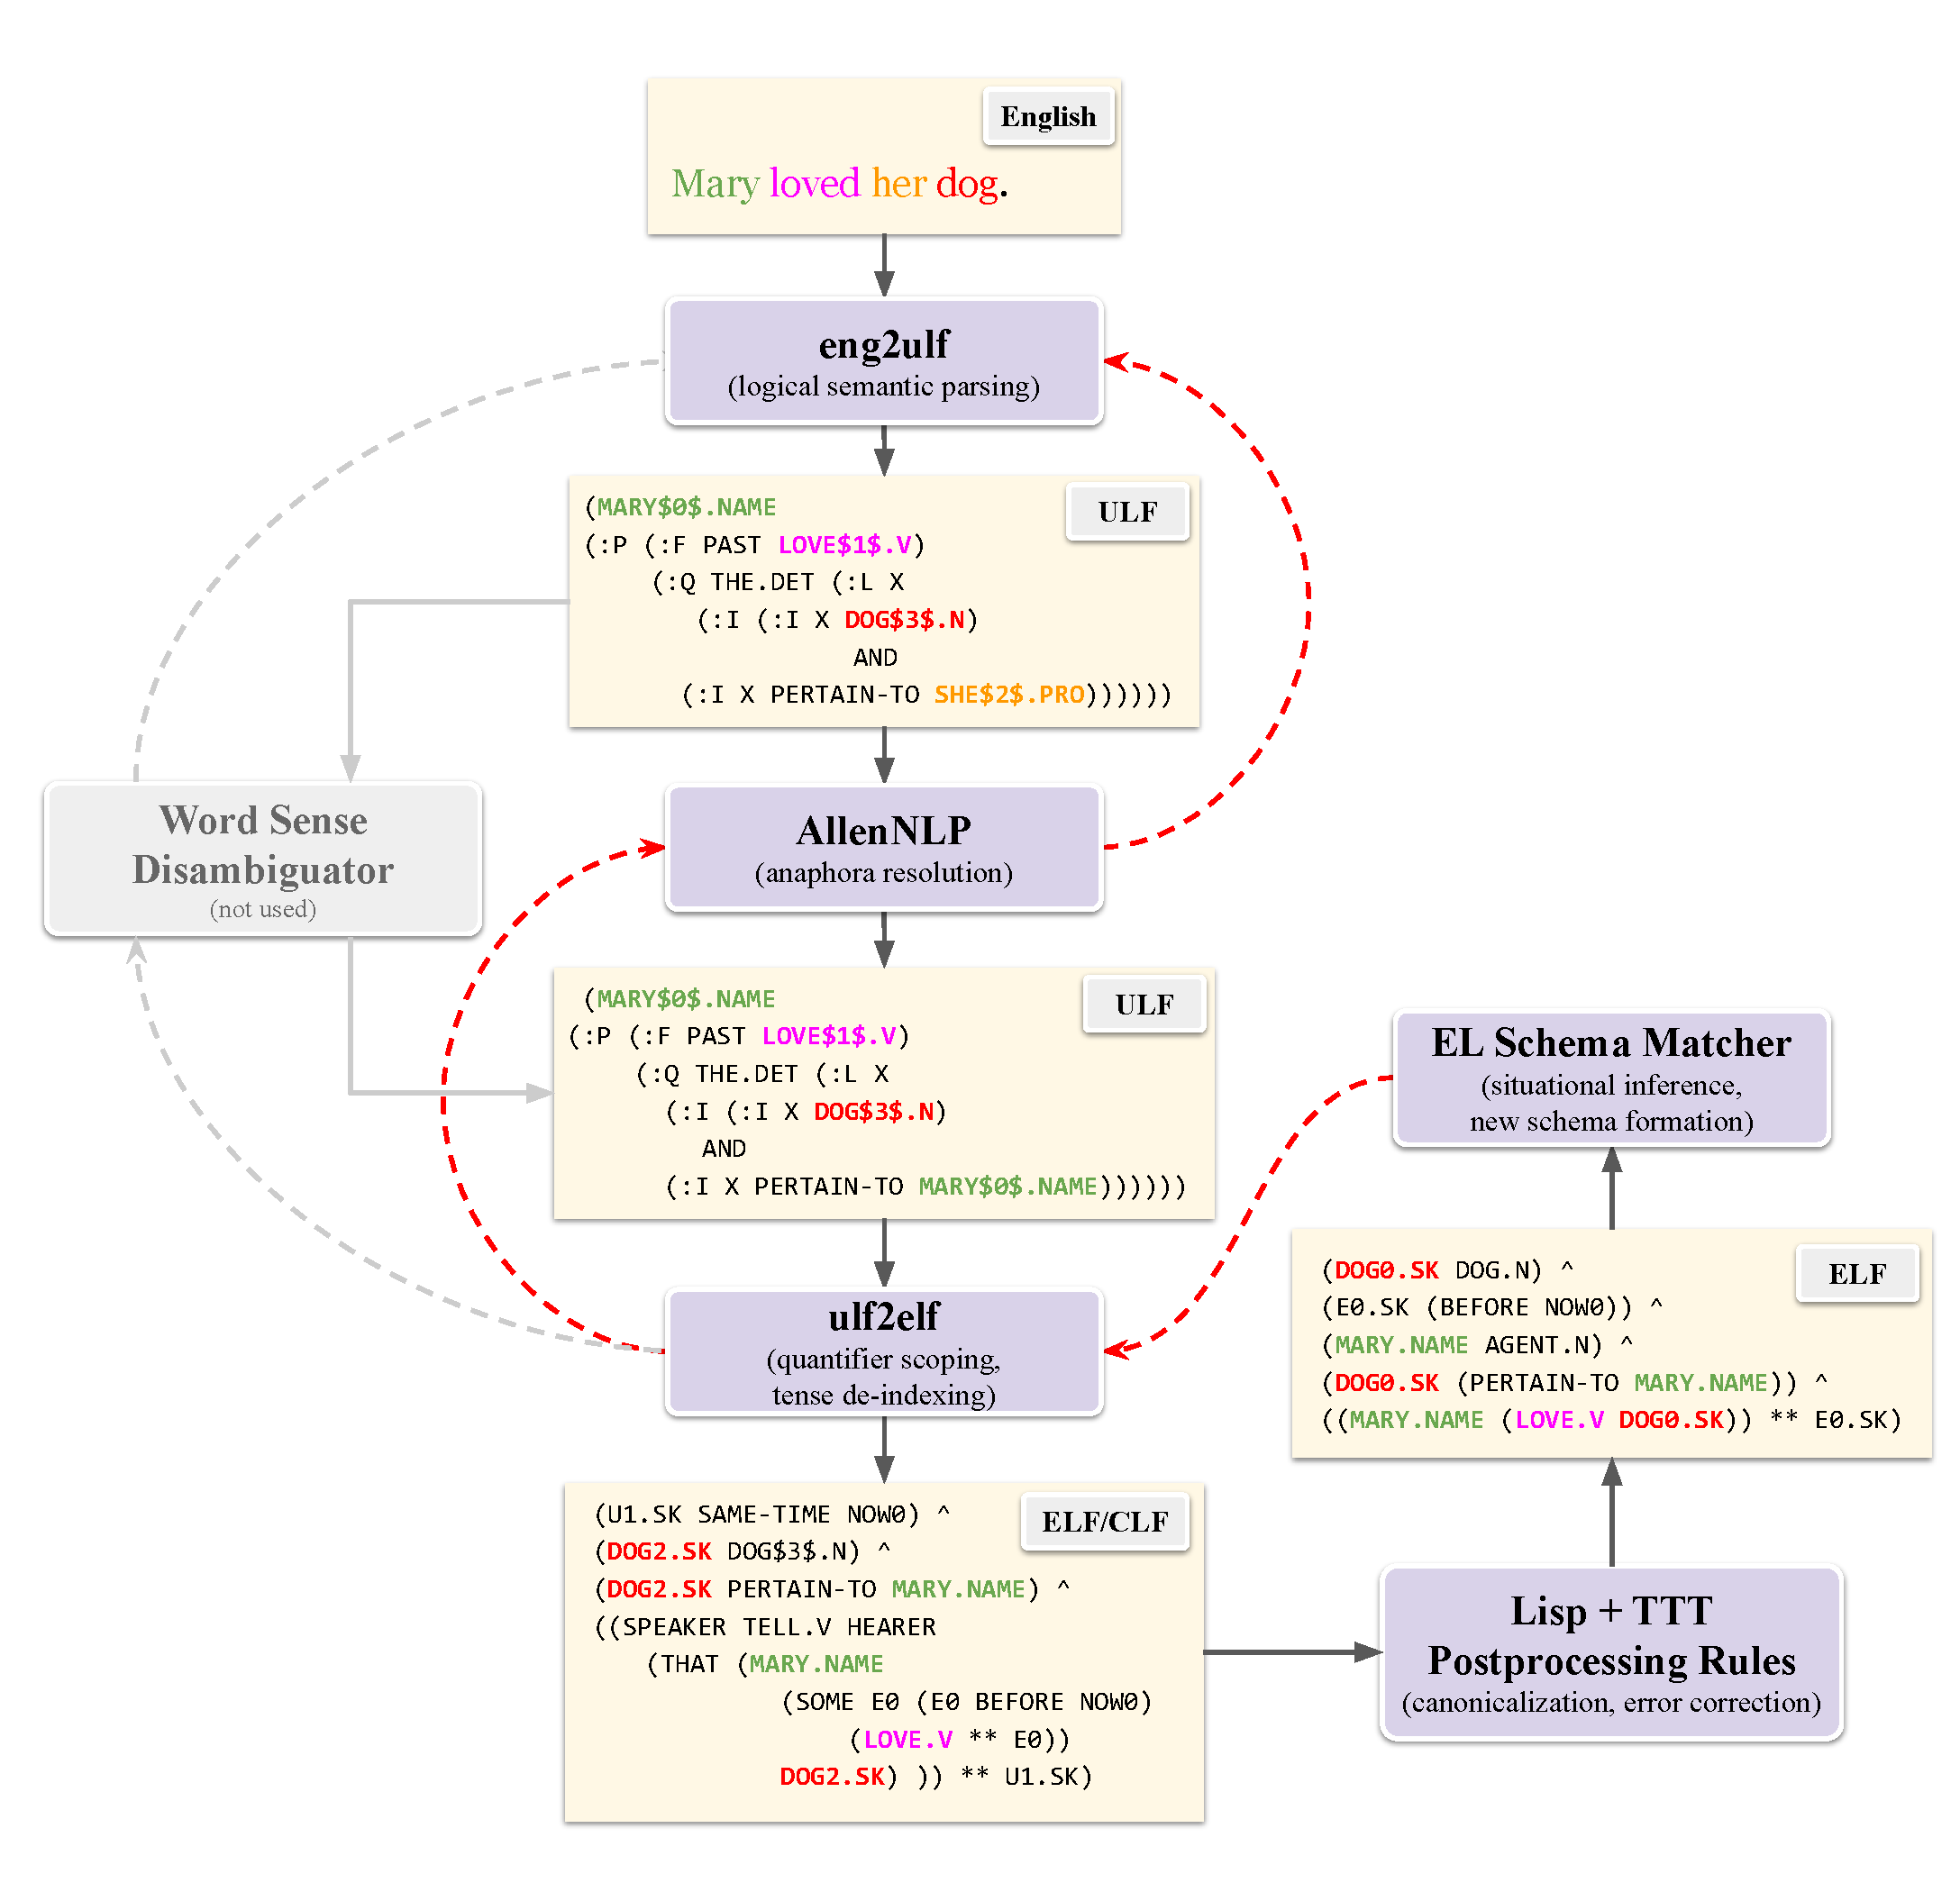
\includegraphics[width=\columnwidth]{CH2_el/parserstages}
    \caption{The information flow diagram of the schema project's EL parser. Rounded, purple rectangles represent software components in the parser pipeline. Sharp, pale rectangles represent the data flowing between components, and are annotated with a specific example of each stage of the parse. Solid, dark arrows represent the forward flow of information between components. Dashed, red arrows represent \textit{theoretical} backward flow of information, i.e., downstream decisions that may prompt changes in upstream decisions; currently, no backward information flow is implemented in our EL parser.}
    \label{fig:my_label}
\end{figure}

\subsection{Evaluating ELF Parser Correctness}
Given a hand-annotated set of English/ELF pairs, we could evaluate the correctness of a parser using some distance metric between a parsed ELF and a ``gold'' ELF. Absent this dataset, however, we adopt an inductive definition of ELF correctness based on a similar definition of ULF correctness and several other measures of correctness for the remaining pipeline steps. The components of a parsed ELF's correctness are as follows:

\begin{enumerate}
    \item The correctness of the parsed ULF.
    \item The accuracy of the word sense disambiguation step, which we take to be $0\%$, as we chose to consider this problem out-of-scope for the current phase of the EL schema project.
    \item The accuracy of the anaphora/coreference resolution step, for which we adopt the accuracy measurements of the underlying coreference analysis engine integrated into the EL parsing pipeline.
    \item The accuracy of quantifier scoping.
    \item The accuracy of canonicalization, which we conservatively define to be the proportion, evaluated on a set of held-out stories, of final ELFs that conform to the grammar given by Figure~\ref{fig:el_cfg}.
    \item The accuracy of tense de-indexing., which is not explicitly known; tense de-indexing is performed using the implementation of tense trees \citet{schubert1990tensetrees}, and no correctness evaluations on any corpora were produced for that method, which relies on qualitative arguments of correctness. However, our implementation of tense tree de-indexing does not include temporal adverbial de-indexing, and so formulas with temporal adverbials can be assumed to be incorrectly de-indexed.
\end{enumerate}

\begin{figure}
    \centering
    \newcolumntype{L}{>{$}l<{$}}
\newcolumntype{R}{>{$}r<{$}}

\newcommand\LP{\texttt{(}}
\newcommand\RP{\texttt{)}}
\newcommand\SP{\hspace{0.2mm}}
\newcommand\AZ{\texttt{[A-Z]}}

\small
\begin{tabular}{|L|}
\hline\\
{\setlength\tabcolsep{8pt}
\begin{tabular}{L R L}
%\begin{longtable}{L R L}
\phi &\Coloneqq &\phi_{atom}\\
&| &\texttt{(not}~\phi\texttt{)}\\
&| &\texttt{(or}~\phi^{+}\texttt{)}\\
&| &\texttt{(and}~\phi^{+}\texttt{)}\\
&| &\texttt{(if}~\phi~\hspace{0.2mm}~\phi~\texttt{)}\\
&&\\
\phi_{atom} &\Coloneqq &\texttt{(}~I~\hspace{0.2mm}~P~\texttt{)}\\
&| &\texttt{(}\phi~\texttt{**}~I\texttt{)}\\
&| &\LP~M~\SP~\phi~\RP\\
&| &\LP~I~\SP~P~\SP~I^{+}~\RP\\
&&\\
I_{lex} &\Coloneqq &[0-9]^{*}\\
&| &\texttt{[A-Z]}^{*}.\texttt{SK}\\
&| &\texttt{[A-Z]}^{*}.\texttt{PRO}\\
&| &\texttt{[A-Z]}^{*}.\texttt{NAME}\\
&| &?\texttt{[A-Z]}\\
&&\\
I &\Coloneqq &I_{lex}\\
&| &\LP~\texttt{K}~\SP~P~\RP\\
&| &\LP~\texttt{KA}~\SP~P~\RP\\
&| &\LP~\texttt{KE}~\SP~\phi~\RP\\
&| &\LP~\texttt{THAT}~\SP~\phi~\RP\\
&| &\LP~\AZ.\texttt{F}~\SP~I^{+}~\RP\\
&| &\LP~\texttt{[A-Z].DET}~\SP~P~\RP\\
&| &\LP~\texttt{SET-OF}~\SP~I^{+}~\RP\\
%\end{longtable}}
\end{tabular}}
{\setlength\tabcolsep{8pt}
\begin{tabular}{L R L}
%\begin{longtable}{L R L}
P_{atom} &\Coloneqq &\AZ.\texttt{N}\\
&| &\AZ.\texttt{V}\\
&| &\AZ.\texttt{A}\\
&| &\AZ.\texttt{P}\\
&| &\LP~\lambda~\SP~\LP~\AZ~^{*}~\RP~\SP~\phi~\RP\\
&| &\LP~\texttt{PASV}~\SP~\AZ.\texttt{V}~\RP\\
&&\\
P &\Coloneqq &P_{atom}\\
&| &\LP~P~\SP~I^{+}~\RP\\
&| &\LP~M~\SP~P~\RP\\
&&\\
M &\Coloneqq &\AZ.\texttt{ADV-[AEFS]}\\
&| &\LP~\texttt{ADV-[AEFS]}~\SP~P~\RP\\
&| &\LP~\texttt{ADV-[AEFS]}~\SP~M~\RP\\
&| &\texttt{PLUR}\\
\end{tabular}}\\
\vspace{0.2mm}\\
\hline
\end{tabular}
%\end{longtable}}
    \normalsize
    \caption{A context-free grammar representing the simplified Episodic Logic language used for EL schemas. $\phi$ and $\phi_{atom}$ are the rules for forming composite and atomic propositions, respectively; $P$ and $P_{atom}$ are similar rules for complex and atomic predicates. $M$ is a rule for forming predicate modifiers, and $I$ is a rule for forming domain individuals in the EL ontology. The atomic individual rule, $I_{lex}$, may form names, pronouns, Skolem constants, numbers, and variables.}
    \label{fig:el_cfg}
\end{figure}

\subsection{ULF-to-ELF Conversion}
In converting ULFs to ELFs, we adapt the implementation of the EL parser given by \citet{schubert-2014-treebank} to accept pre-formed ULFs rather than creating its own from Treebank parses. Having separated ULF into a prior pipeline step, we refer to this modified parser as \texttt{ulf2elf}. \texttt{ulf2elf} handles quantifier scoping, tense de-indexing, and some canonicalization steps.
%We discuss those steps here.

%\subsubsection{Utilizing Syntactic Information}
%ULF's proximity to the linguistic form of English imbues it with syntactically-derived information that may be absent in the final, more abstract EL form.
Although canonicalization and post-processing of the ELFs, detailed in \ref{subsec:postproc}, are typically performed after arriving at ELFs, some transductions must be performed, or noted down for later performance, at an earlier stage in the pipeline with access to this syntactic information in the ULFs.
%For example, the predicate-argument structure of the sentence \textit{``Kim used to sleep.''}, and its corresponding ULF \texttt{(KIM.NAME ((PAST USE.V) (KA SLEEP.V)))}, centers around the root verb predicate, \el{USE.V}, which is parsed into past tense and assigned the reified kind-of-action argument \el{(KA SLEEP.V)}.
%The de-indexing algorithm used to decode explicit event times from grammatical tense will transmute this syntactic form into the final ELFs \texttt{\texttt{(E1.SK BEFORE NOW1)} and \texttt{((KIM.NAME (USE.V (KA SLEEP.V))) ** E1.SK)}}.
%Recovery of the original syntax is difficult from this ELF: its source sentence might have been \textit{``Kim used to sleep.''}, but might also have been \textit{``Kim was using [the action of sleeping].''}, whose past progressive tense implies a totally different semantics.
%Therefore, we normalize the \textit{used to} form during the ULF stage, converting it 
%Another example is the effect of pronoun choice on quantifier scoping.
%During ULF-to-ELF conversion, possessive pronoun determiners, e.g. \texttt{(HER.D TOY.N)}, are transmuted into lambda predicates under the scope of the pronoun's referent, e.g. \texttt{(THE.D (L X ((X TOY.N) AND (X PERTAIN-TO \textbf{Y}))))}, where the referent, \texttt{\textbf{Y}} is resolved later.
%Because the scope of Y is not known---it could be universally quantified, as in \textit{``Every girl loves her toy.''}---


\subsubsection{Quantifier Scoping}
% state left-to-right order assumption.
% (Len email has justification involving determiners)

\subsubsection{Tense De-Indexing}
% calculate lower bound of correctness: sentences with only one tense and no temporal adverbs
% calculate upper bound of correctness: sentences with no temporal adverbs

\subsection{Anaphora Resolution}
\label{sec:anaphora_res}

Two kinds of anaphora resolution are performed in EL parsing: \textbf{entity resolution}, in which co-referring entities are merged, and \textbf{predicate resolution}, in which untyped words that refer to previously introduced predicates are re-typed with those predicates. An example of predicate resolution is found in the phrase ``a new one'', in which the type of the object represented by the noun ``one'' is undetermined: a new one of what? Both kinds of resolution are performed using the AllenNLP library's co-reference resolution tool \citep{Gardner2017AllenNLP}, which itself solves only the entity resolution problem by identifying co-referring clusters of spans of token indices. Because token indices are also known for EL predicates (and some individuals, like names, introduced directly by the text), we identify individuals in the logical domain with type predicates whose indices exist inside spans identified by AllenNLP. These spans may identify multiple individuals or predicates in the ELFs, e.g. ``her iPhone'', whose span nests both the individual ``her'' and the individual ``iPhone''. However, each component individual of such a span will have its own one-width span in its own co-reference cluster, and so this aliasing problem is averted by processing co-reference spans in order of increasing width.

\begin{figure}
    \centering
    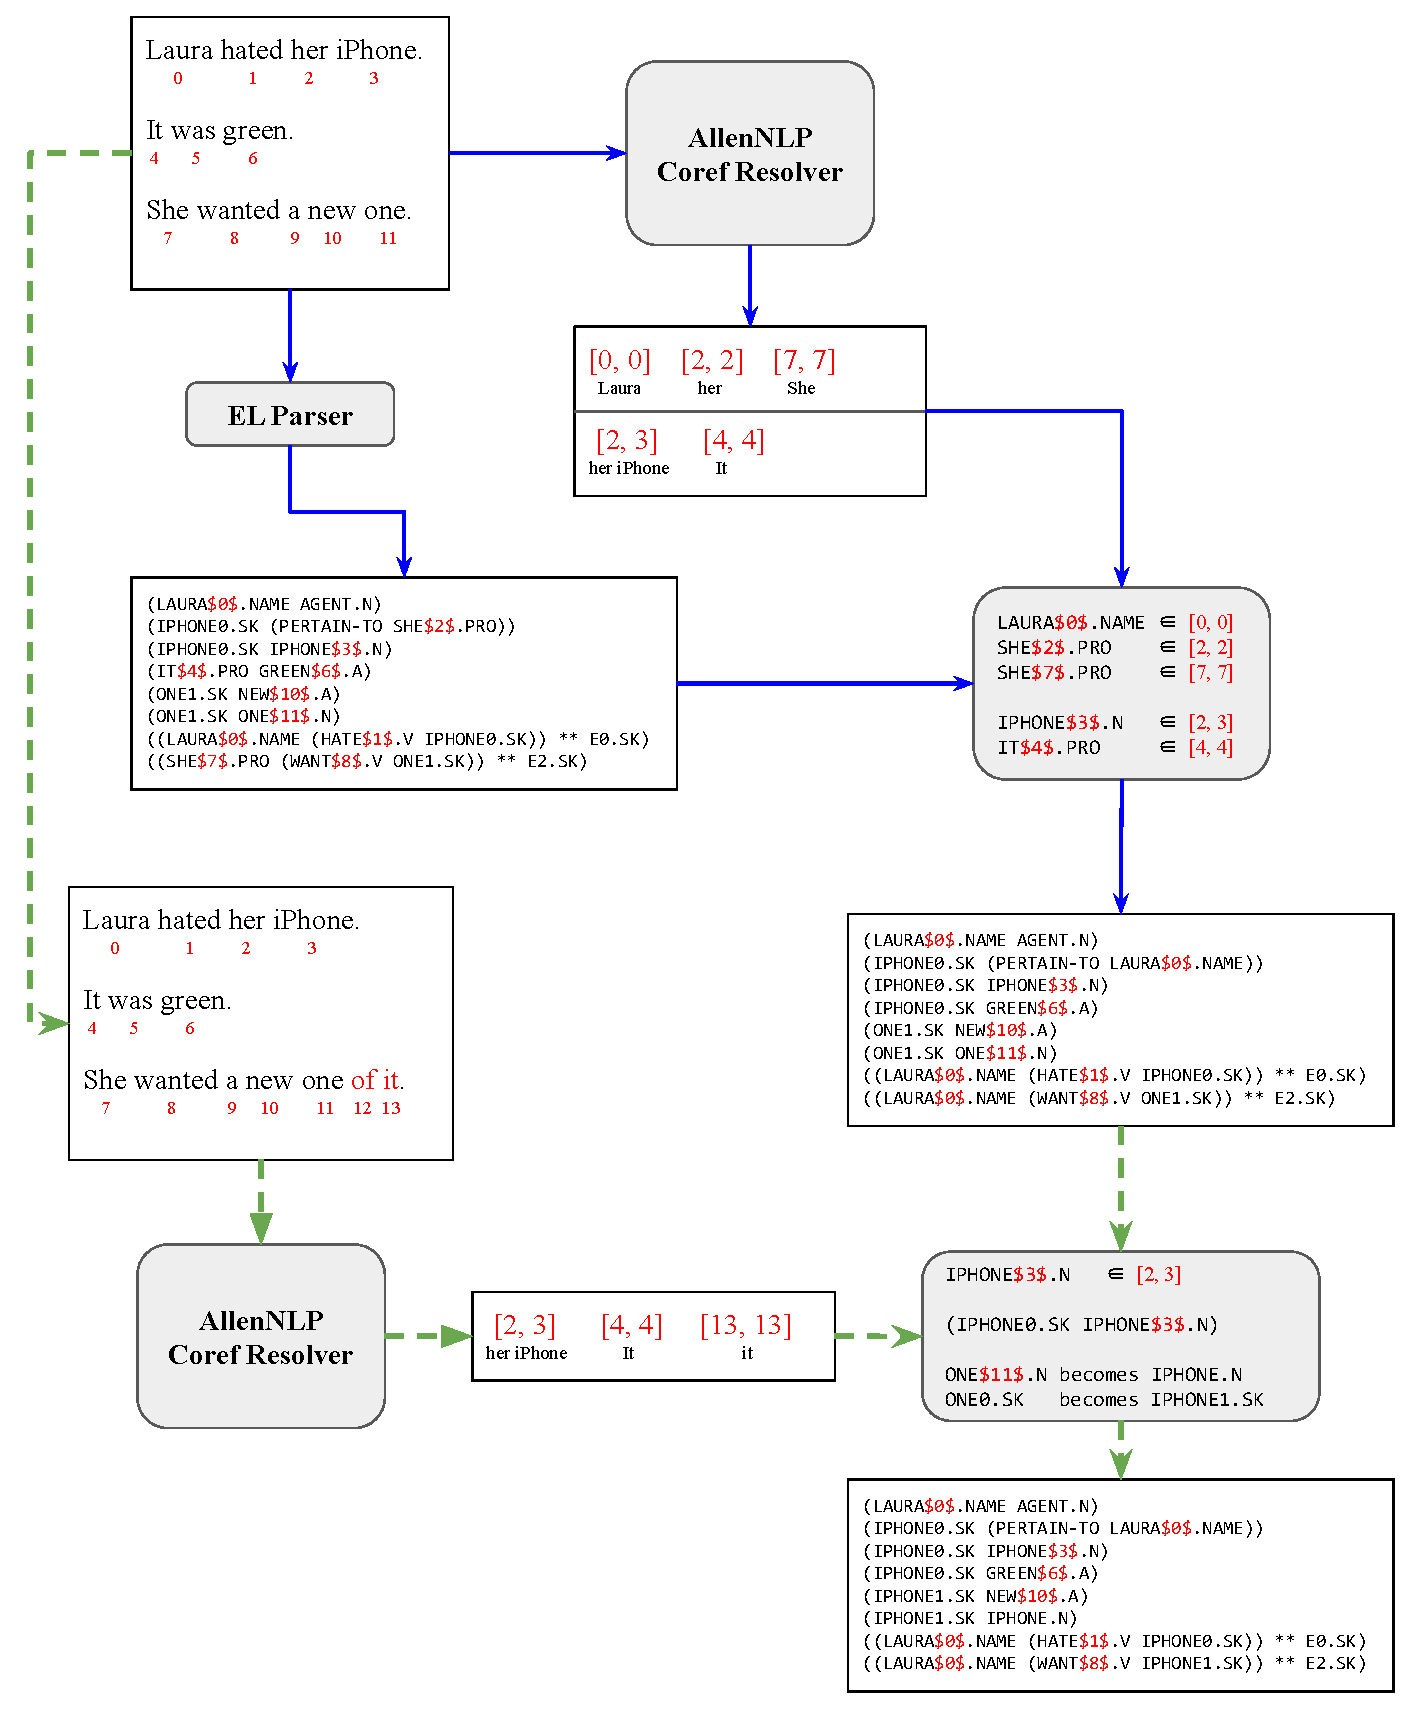
\includegraphics[width=0.99\columnwidth]{CH2_el/coref_fig.pdf}
    \caption{An illustration of the anaphora resolution stage of EL parsing described in Section~\ref{sec:anaphora_res}. Solid blue arrows denote steps of \textbf{entity resolution}, in which co-referring entities are merged. Dashed green arrows denote steps of \textbf{predicate resolution}, in which a referred-to predicate is identified and applied to a distinct entity.}
    \label{fig:coref_process}
\end{figure}

The only predicate anaphora we currently handle are those where the referring word is ``one'', as in ``a new one''. To handle this, we alter the source text by replacing any noun-tagged ``one'' with the string ``one of it''. We then once again perform entity resolution as described above, only identifying the cluster to which the newly introduced ``it'' belongs. The type predicates describing individuals in that cluster are then extracted from the EL parse and applied to the original EL parse's ``one'' individual, whose \el{ONE.N} predicate is then removed, and whose Skolem name is re-calculated from its new predicates. The predicate resolution step occurs after the entity resolution step.

\subsection{Word Sense Disambiguation}
We do not currently perform word sense disambiguation in our EL parser due to the downstream use case of EL schema learning; EL schemas aim to provide a full situational context for each action, and so word senses, which aim to clarify the action represented by a verb, are not necessary when schemas are fully fleshed out with semantic types for all arguments and other relevant context. Annotating verbs with word senses in an error-prone way risks contradicting the actual context within the schema. If word senses are still required after schema learning is complete, the context provided by each schema will hopefully provide even more information to pick senses, whereas little information will have been lost from the original text. During protoschema-based learning, which we describe in Sections~\ref{sec:protoschemas}~and~\ref{sec:lome}, we use neural methods that implicitly assess word sense based on sentential context to pick the best matching protoschema.

\subsection{Post-processing}
\label{subsec:postproc}
The final ELFs obtained from the existing ULF-to-ELF transduction implementation by \citet{schubert-2014-treebank} are not immediately suitable for use in the schema system; the complex, nested formulas that \texttt{ulf2elf} outputs often require further breakdown and Skolemization to align with the simple, canonicalized formulas found in EL schemas. The simplified EL grammar we assume within the schema system is given by Figure~\ref{fig:el_cfg}; this grammar defines what a ``correct'' EL formula is in the context EL schemas. Even without assuming such a restrictive grammar, however, \texttt{ulf2elf} still introduces a significant number of errors into its output ELFs. Fortunately, however, as \texttt{ulf2elf} is a deterministic, rule-based program, many error types can be classified into patterns and fixed with additional post-processing rules, which we describe here.

We post-process \texttt{ulf2elf} output formulas by iteratively applying two sets of rules---one set written in Lisp and the other implemented as a set of TTT transductions---until a full iteration passes with no changes made. Though more computationally expensive, the Lisp post-processing rules allow for more complicated fixes than TTT would. All of the rules, regardless of implementation, fall into one of the following four categories:

% TODO: rewrite the following subsubs; they're pasted from an email I wrote to Len
\subsubsection{Canonicalization Rules}
These rules perform top-level Skolemization, conjunction splitting, lambda-predicate splitting and removal, normalization of parentheses, re-arrangement of sentential operators and modifiers, and other similar transductions meant to reduce the size and standardize the form of complex ELFs. These rules were developed with the theory and literature of EL in mind, and were not crafted to improve performance on a development story corpus.

\subsubsection{Error Correction Rules}
Rules that fix strange artifacts of the imperfect parsing, whether ULF or ELF parsing, up to that point; some formulas just come out in invalid ways but in identifiable patterns, so rules can be written for them. These were developed on a dev set of stories and evaluated on a test set of stories to see how many invalid ELFs were made valid. They're highly technical and granular.

\subsubsection{Simplifying Rules}
Rules that convert formulas into equivalent and/or more meaningful ones, like "There~is~X"~$\Rightarrow$~"X~is", or, in the case of a less equivalent but more useful transduction, the removal of progressive markers from verbs to make sure they play nicer with the simple event schemas. Some of these rules, like the progressive removal rule, have semantic compromises in order to minimize the already massive engineering effort required to get ELFs to match between schemas and stories. These were developed on a dev set of stories.

\subsubsection{Schema-Specific Rules}
Rules that do things that are just nice for schema learning. One example is adding (X AGENT.N) to stories where X is a lexical name or personal pronoun. Another example is shifting past-tense stories forward in time to "NOW", because past-tense stories only have (BEFORE NOW\#) as their deindexing relations, which ends up not imposing any ordering constraints between the story episodes; I convert these to AT-ABOUT, effectively making the story present-tense, to get that ordering. These were developed without reference to any specific story corpus, and mostly just occurred to me as I was programming.

\iffalse
This section describes the means by which we parse Episodic Logical Forms (ELFs) from English sentences. When constructing the parser, we opted not to construct an explicit dataset of ELF/English pairs, as is customary in many semantic parsing endeavors. Instead, we exploit the structure of the EL parsing pipeline (Figure~\ref{fig:el_pipeline}), in which most semantic parsing is handled by the ULF parser. Because a hand-annotated ULF/English dataset \citep{kim2019IWCS} and several ULF parsers \citep{kim2021transition,kim2021naloma} already exist, we can implement only those remaining steps necessary to obtain the final ELFs.

In Section~\ref{subsec:ulf}, we describe and compare existing ULF parsers, including a novel language model-based parser developed as part of the schema project. Then, in Section~\ref{subsec:elparsing}, we discuss the processing steps necessary to obtain ELFs from ULFs.
\fi

%\section{Schema Syntax and Semantics}

%\section{Protoschemas}